\documentclass[12pt]{article}
\usepackage{amsmath}
\usepackage{graphicx}
\begin{document}
\title{Software Requirements Specification\\
Electronic Marking System}
\author{By: \\ Juandre Barnard - 11061015 \\ Melany Barnes - 12030466 \\ Christo Brits - 11080923 \\ Po-Han Chiu - 11063612 \\ Priscilla Hammond - 11025477 \\ Maret Stoffberg - 11071762 \\ \\ For: \\ Jan Kroeze \\ (Computer Science Department - University of Pretoria) \\ \\ Version 1 \\}
  \maketitle   \pagebreak
  \tableofcontents
  \pagebreak
  % 1
  \section{Introduction}
  \paragraph*{The purpose of this document is to illustrate to the client the requirements of the project and reach an agreement between the developers and the client for the scope of the project. This document states clearly what the developed system must be able to do and what functions the system cannot do. This document is regarded as an official contract between the developers and the client when the pre and post conditions stated are met. This document is formulated using LaTeX, Use Case Diagrams, Activity Diagrams and UML Class Diagrams.}
  %2
  \section{Vision}
  \paragraph*{The aim of this project is to provide a mobile web-based marking IT solution to the client, Mr Jan Kroeze from the Computer Science Department at the University of Pretoria, that allows users to upload student marks to a mark sheet and also be able to use/view these marks at a later stage. The solution is aimed to be easy to use and more efficient than the pen-and-paper marking system.}
  % 3
  \section{Background}
  \paragraph*{Currently the course module, COS 222, offered by the Computer Science Department, University of Pretoria, uses a pen-and-paper system to mark their student's practicals. During a practical marking session, markers give the students a piece of paper to write their own name and student number on. The marker then writes the mark obtained by that student on that piece of paper. Only after all students have had their practicals marked, will all the marks written on different pieces of paper be digitalized and submitted for use by the lecturer. From this system, the client sees the opportunity to use an IT solution for the markers to directly submit the marks electronically to a database, where the lecturer stores the marks, when the markers are marking the practicals. This reduces the potential risk of student marks being lost before it is recorded electronically. This also reduces the use of paper during each practical marking session, saving trees. The idea of using the Android platform is because it is assumed that tutors are most likely in possession of an Android OS Smartphone, so there will be no hardware issues. It is also assumed that there are wifi-hotspots in the Informatorium, University of Pretoria, where the practical marking sessions are assumed to take place, so there will be no internet connection issues.}
  %4
  \section{Architecture requirements}
  % 4.1
  \subsection{Access channel requirements}
  \paragraph*{Lecturers, tutors and students will access this system's services through a Mobile Android application. They will also be able to use this system's services through a web browser interface. A lecturer will be able to manage the marks and will be able to upload/extract mark lists as CSV files.}
  % 4.2
  \subsection{Quality requirements}
\begin{description}
  \item[Auditability:] \hfill  \\
  \textbf{•(Source: Jan Kroeze, Priority: Critical, Requirement: NFRQ1) \\
  Everything that happens on the system must be saved in a log and must be able to be queried. Especially alterations to marks will be logged. Any updates made as well as additions added will be logged.} \\
  \item[Flexibility:] \hfill \\
  \textbf{•(Source: Jan Kroeze, Priority: Important, Requirement: NFRQ2) \\
  The application will work on Mobile phones with an Android operating system. The web interface will be able to be viewed from a mobile device or from a personal computer.}\\
  \item[Reliability:] \hfill \\
  \textbf{•(Source: Jan Kroeze, Priority: Critical, Requirement: NFRQ3) \\
  The application will always be on line and will be usable as long as users are connected to the internet, same applies to the web interface. If the user loses internet connection the system will make a local backup on the device being used and will commit this data to the system as soon as it gets internet connection again.}\\
  \item[Scalability:] \hfill \\
  \textbf{•(Source: Jan Kroeze, Priority: Critical, Requirement: NFRQ4) \\
  The system needs to react quickly on input or commands. Performance and reliability should not be dependent on the amount of users on the system.}\\
  \item[Security:] \hfill \\
  \textbf{•(Source: Jan Kroeze, Priority: Critical, Requirement: NFRQ5) \\
  Users will have to log in with their specific user name and password to access the system. Only valid users, with valid authentication and presence on the system may gain access to the system. Lecturers will be able to change closing times of mark sheets, change marks and view reports. Markers will be able to input student marks which he is assigned to. Students will only be able to view their own marks.} \\
  \item[Usability:] \hfill \\
  \textbf{•(Source: Jan Kroeze, Priority: Important, Requirement: NFRQ6) \\
  It must be a simple, easy to use system.}
\end{description} 
  % 4.3
  \subsection{Integration requirements:}
  \paragraph{All the data will be imported into the system via a CSV file.}
  \paragraph{The database will be updated in real time. Meaning when a mark sheet is opened, the relevant data will be uploaded to the application or web interface from the database and thus as a mark is entered by a marker, the system will be updated.}
  \paragraph{Critical Protocols that needs to be used are:
  SOAP - Used for exchanging structured information.
  LDAP - Used for accessing and maintaining distributed directory information.
  SMTP - Used for electronic mail transmission.
  Combining these protocols will facilitate reliability, security and auditability.}
  \paragraph{Since speed is critical, the files used to update the database will be as small as possible. This also increases scalability.}
  % 4.4
  \subsection{Architecture constraints}
  \paragraph{
  The technologies that must be used are:
  }
  \begin{itemize}
  \item \textbf{•Python, Django}
  \item \textbf{•Android}
  \item \textbf{•SQL}
  \item \textbf{•HTML 5}
  \item \textbf{•CSS 3}
  \item \textbf{•CSV}
  \item \textbf{•Pdf}
  \item \textbf{•MVC - Software Pattern}
\end{itemize}
  % 5
  \section{Functional requirements}
  % 5.1
  \subsection{Introduction}
  \paragraph{(Source: Jan Kroeze, Priority: Critical, Requirement: FRQ01) \\
  Any registered user should be able to log in and out of the system using a unique username and password. After a user has logged in, he is redirected to his home page.}
  \paragraph{(Source: Jan Kroeze, Priority: Critical, Requirement: FRQ02) \\
  A student must be able to view their marks on the application as well as on  the web interface. The student can then view each module's marks separately via links to each module. }
  \paragraph{(Source: Jan Kroeze, Priority: Critical, Requirement: FRQ03) \\
  A marker, has additional links to the modules he marks. When a marker click on these links, the active mark sheet of the module is displayed. The marker can then click on the mark sheet to open the mark sheet and enter marks. When the marker open the mark sheet he has to enter the students initials, surname, full name, student number or username. The system has to use autocomplete search for this function. The marker then may view, delete add or modify the marks. Afterwards he has to save and close the mark sheet.}
  \paragraph{(Source: Jan Kroeze, Priority: Critical, Requirement: FRQ04) \\
  On a lecturer's home page, a list of all his existing mark sheets is displayed. On the home page, he may either create a new mark sheet, or view an existing mark sheet. An existing mark sheet can be viewed by searching or by selecting one out of the list.}
  \paragraph{(Source: Jan Kroeze, Priority: Critical, Requirement: FRQ05) \\
  To create a new mark sheet, the lecturer of a module must have a [New Mark Sheet] button. For each new mark sheet, the lecturer should be able to enter a description, question amount with a maximum amount of marks per question, a rubric, marker's privileges, expiry date and release date. The marking privileges refer to who may enter or change marks, the default should be the lecturer only. The expiry date refer to when the mark sheet is locked, meaning no more marks may be entered. The release date refer to when the student may view their marks, the default is the expiry date. After all the details are entered, there must be a form of confirmation like a [confirm] button.}
  \paragraph{(Source: Jan Kroeze, Priority: Critical, Requirement: FRQ06) \\
  When viewing a mark sheet, the lecturer may choose to unlock the mark sheet. The lecturer may then modify the marks on the sheet. The lecturer must save the mark sheet and lock it. }
  \paragraph{(Source: Jan Kroeze, Priority: Critical, Requirement: FRQ07) \\
  When viewing a mark sheet, the lecturer may export the mark sheet in either CSV or PDF file. He may also choose to delete the mark sheet}
  \paragraph{(Source: Jan Kroeze, Priority: Important, Requirement: FRQ08) \\
  The lecturer should be able to view statistics of a mark sheet.  This report must be exportable as a pdf. This includes the percentages that passed and has extinctions, as well as the average and standard deviation. The report also include a distribution graph, pie chart and bar graph.}
  \paragraph{(Source: Jan Kroeze, Priority: Important, Requirement: FRQ09) \\
  The system must be able to calculate compositional marks.}
  \paragraph{(Source: Jan Kroeze, Priority: Critical, Requirement: FRQ10) \\
  The system must log all changes made to the mark sheet. This must include a timestamp, the modification and the user involved. Only the lecturer should be able to view the log.}
  \paragraph{(Source: Jan Kroeze, Priority: Nice-To-Have, Requirement: FRQ11) \\
  The system must notify a student when his marks is modified.}
  \paragraph{(Source: Jan Kroeze, Priority: Important, Requirement: FRQ12) \\
  The system must automatically log out after no activity in 60 minutes.}
 % 5.2
  \subsection{Scope and Limitations/Exclusions}
  \begin{center}
  \advance\leftskip-2.0cm
  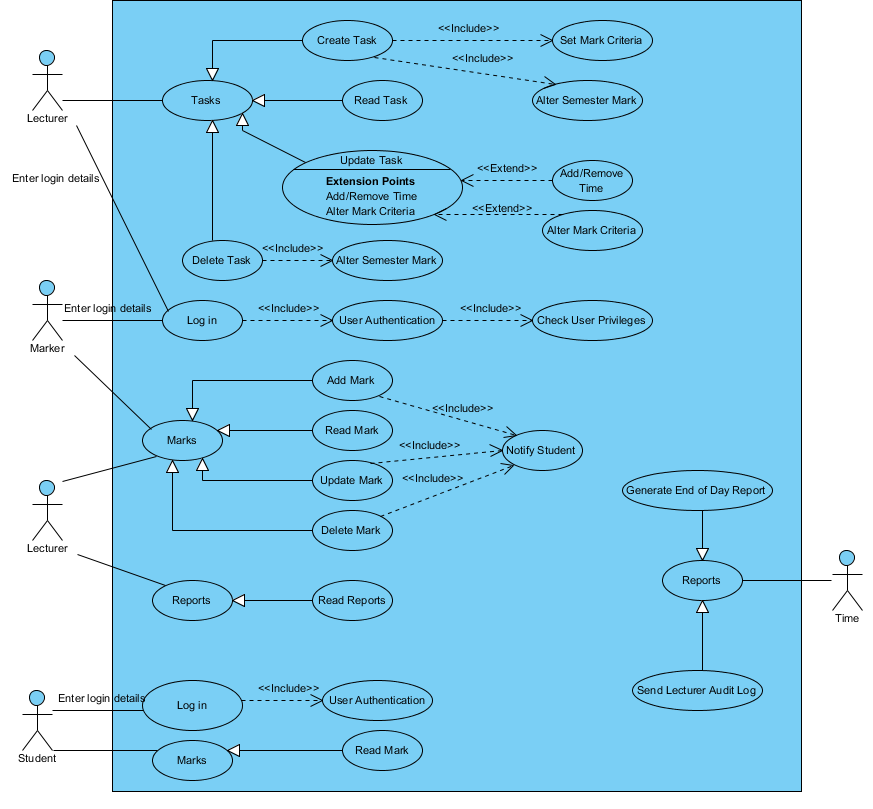
\includegraphics[width=180mm]{UseCaseDiagram1.png}  
  \end{center}
  % 5.3
  \subsection{Required functionality}  
  \begin{center}
  \advance\leftskip-1.0cm
  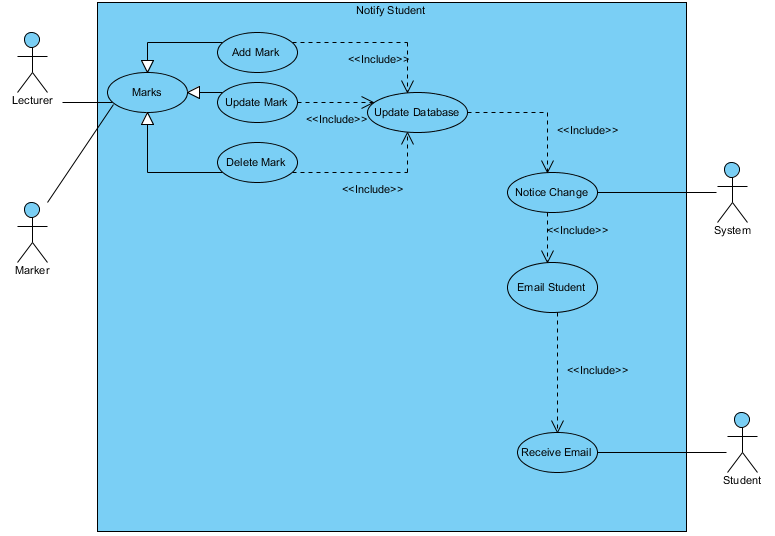
\includegraphics[width=160mm]{UseCaseDiagram2.png}  
  \end{center}
  \begin{center}
  \advance\leftskip-1.3cm
  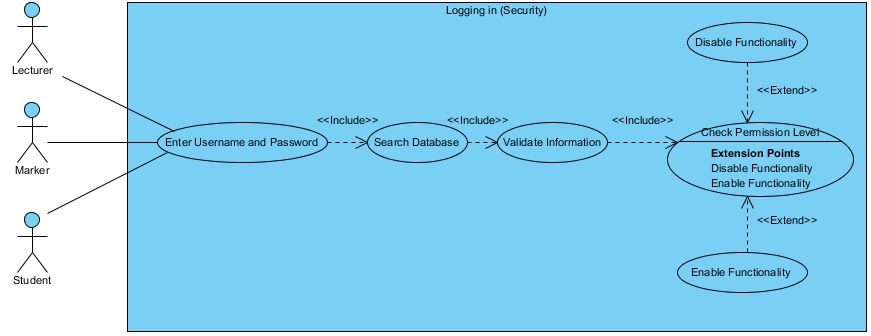
\includegraphics[width=160mm]{UseCaseDiagram3.png}  
  \end{center}
  % 5.4
 \subsection{Use case prioritization}
 \paragraph*{Critical Use Cases are the main cases that the system is made up of namely, Logging In, Create Tasks, Create Marks and Generating Reports. Without these cases the system will have limited to no functionality which will lead to a system that is not required by anyone.}
 \paragraph*{Important Use Cases are the cases that improves the critical use cases and introduces a wider variety of functionality. These cases are Read, Update and Delete of Tasks, Read Update  and Delete of Marks.}
 \paragraph*{Nice-To-Have Use Cases make the system more user friendly and provides a better user experience. This case is the Notify Student use case, this is where the system automatically, emails the student of any changes made, either to their marks, namely adding marks, updating marks and deleting marks. This functionality can also be extended to the creation, update and deleting of tasks. This will help the student to stay up to date with what tasks needs to be done in the module.}
 % 5.5
 \subsection{Use case/Services contracts}
 \paragraph*{\underline{Pre-Conditions: }\\ Login - User information is stored in the database.
 \\ Create Task - Lecturer is assigned to the module and the user has the correct permission level.
 \\ Read Task - A task is already created and the user has the correct permission level.
 \\ Update Task - A task is already created and the user has the correct permission level.
 \\ Delete Task - A task is already created and the user has the correct permission level.
 \\ Add Mark - Lecturer or Marker is assigned to the module. Task timeslot is open. A Student is assigned to the corresponding module and task.
 \\ Read Mark - Lecturer, Marker or Student is assigned to the module.
 \\ Update Mark - Lecturer is assigned to the module and the user has the correct permission level.
 \\ Delete Mark - Lecturer is assigned to the module and the user has the correct permission level.
 \\ Generate Report - Lecturer is assigned to the module and the user has the correct permission level.}
 \paragraph*{\underline{Post-Conditions:} \\ Login - User information has been validated.
 \\ Create Task - New task exists and Lecturers and Markers assigned to the module with the correct permission level is able to work with it. Students assigned to the module is notified.
 \\ Read Task - Knowledge is obtained.
 \\ Update Task - Task is now correct and Lecturers and Markers assigned to the module with the correct permission level is able to work with it. Students assigned to the module are notified.
 \\ Delete Task - Task is removed from the system. Students assigned to the module are notified.
 \\ Add Mark - Mark is added to the student's semester mark. Student who received the mark is notified.
 \\ Read Mark - Knowledge is obtained.
 \\ Update Mark - Student's semester mark is updated accordingly. Student who's mark has been updated is notified.
 \\ Delete Mark - Student's semester mark is updated accordingly. Student who's mark has been updated is notified.
 \\ Generate Report - Knowledge is obtained.}
 \begin{center}
  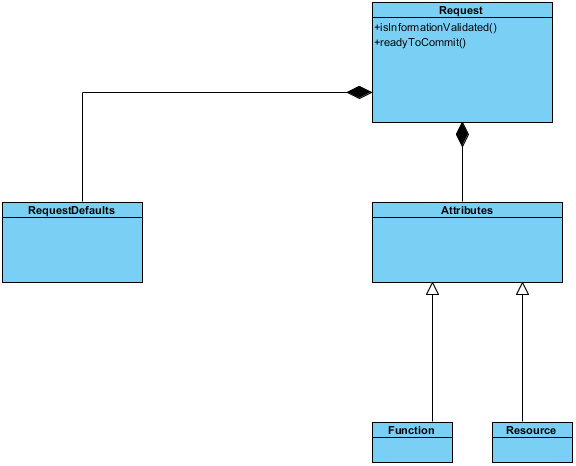
\includegraphics[width=120mm]{Diagram1.png}  
  \end{center}
  \begin{center}
  \advance\leftskip-2.0cm
  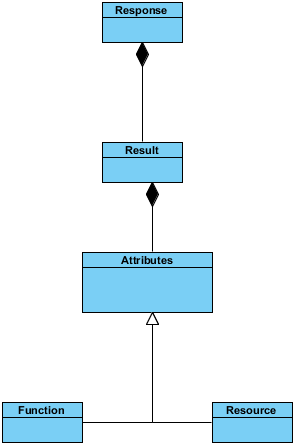
\includegraphics[width=60mm]{Diagram2.png}  
  \end{center}
 % 5.6
 \subsection{Process specifications}
  \begin{center}
  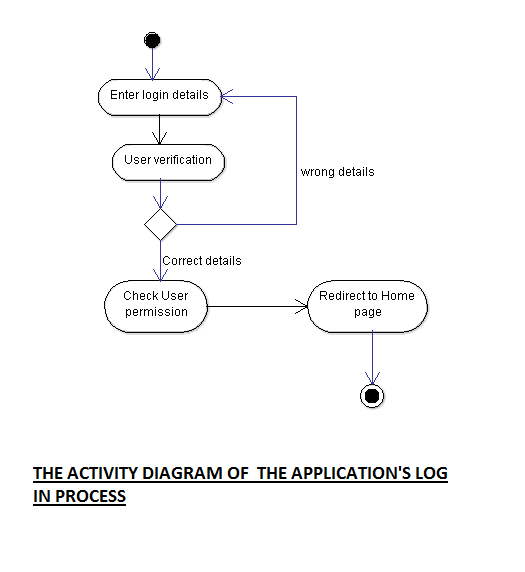
\includegraphics[width=130mm]{UserLogin.png}  
  \end{center}
  \begin{center}
  \advance\leftskip-2.8cm
  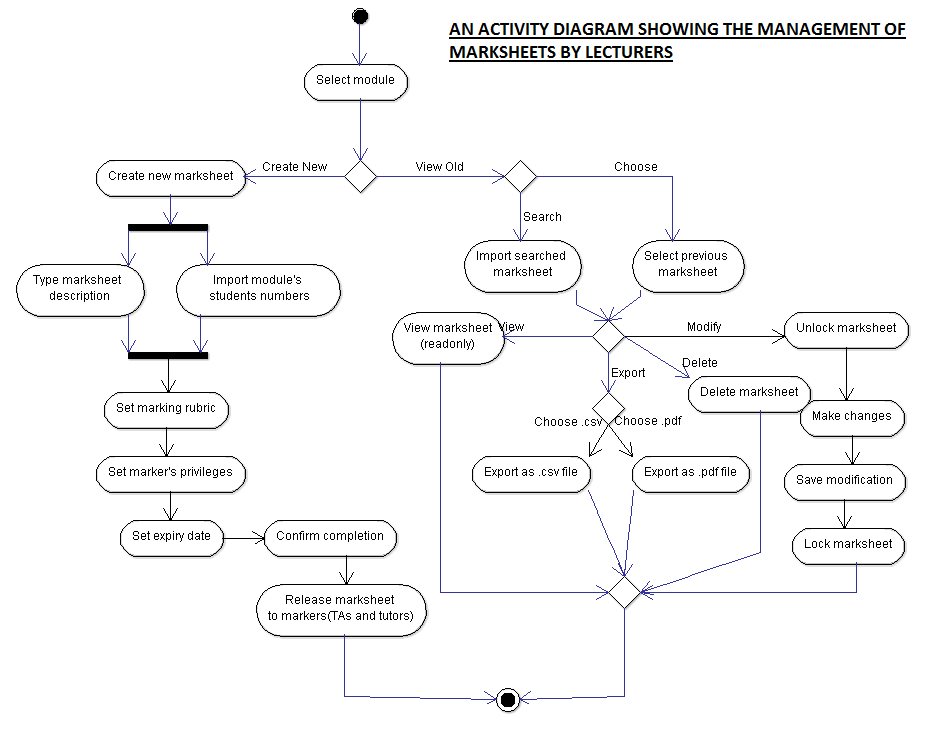
\includegraphics[width=190mm]{LecturersManagingMarksheets.png}  
  \end{center}
  \begin{center}
  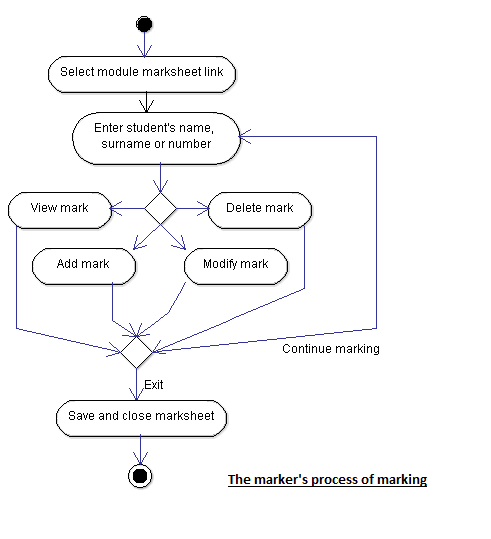
\includegraphics[width=130mm]{Tutorsmarkingmoduleactivities.png}  
  \end{center}
 % 5.7
 \subsection{Domain Objects}
  \begin{center}
  \advance\leftskip-3cm
  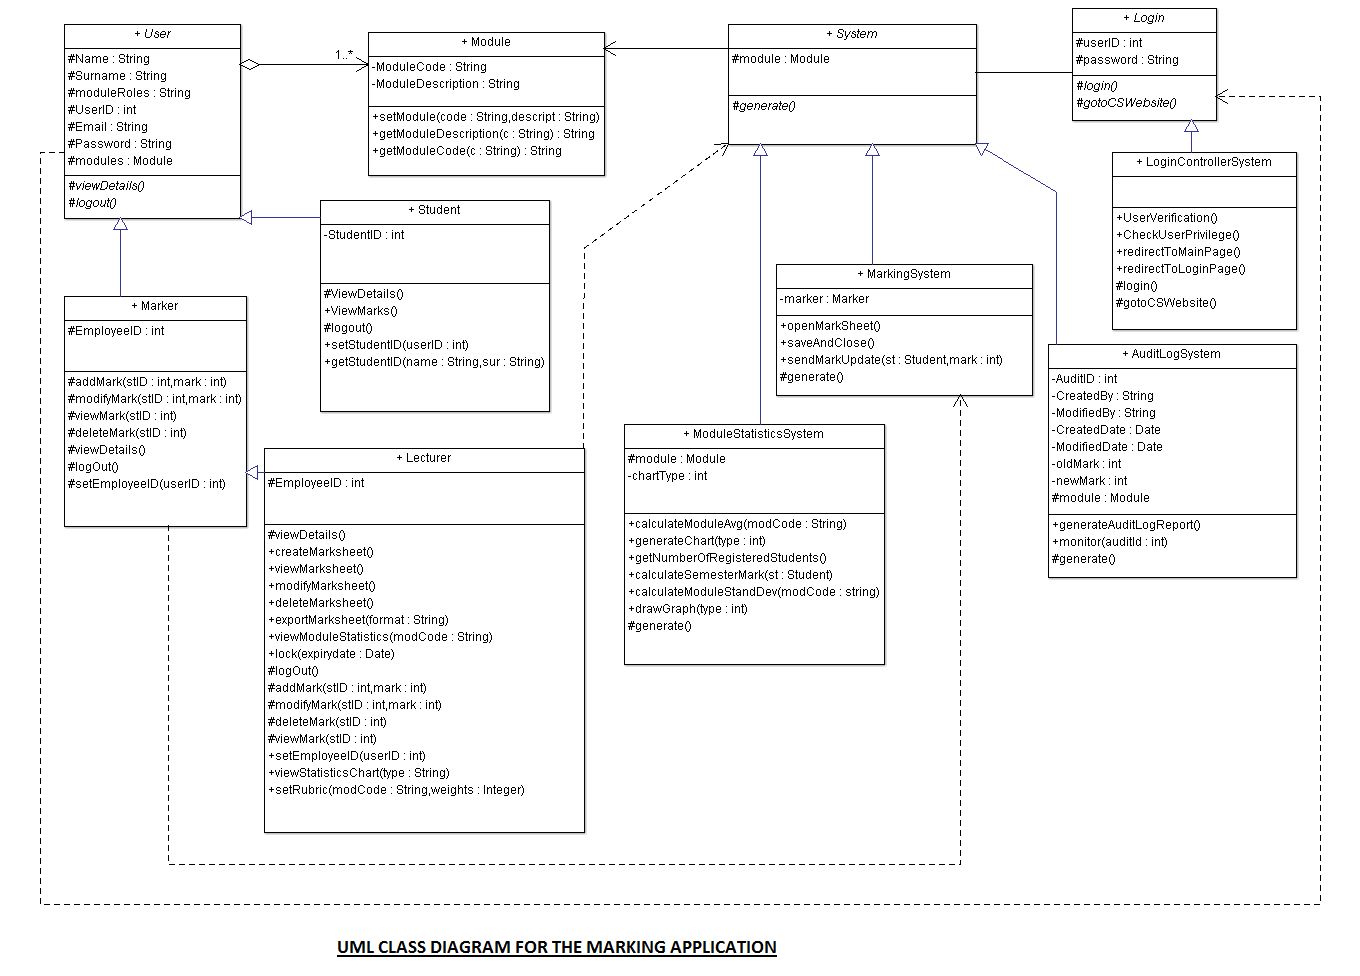
\includegraphics[width=200mm]{UMLTechnologies.png}  
  \end{center}
 % 6
 \section{Open Issues}
\begin{itemize}
  \item \textbf{•Theft/Loss of mobile device}
  \item \textbf{•Cannot be held resonsible if the user does not log off.}
\end{itemize}
 % 7
 \section{Glossary} 
 \begin{itemize}
  \item \textbf{•CSS - Cascading Style Sheets}
  \item \textbf{•CSV - Comma-separated values}
  \item \textbf{•HTML - Hypertext Markup Language}
  \item \textbf{•HTTP - Hypertext Transfer Protocol}
  \item \textbf{•LDAP - Lightweight Directory Access Protocol}
  \item \textbf{•PDF - Portable Document Format}
  \item \textbf{•SOAP - Simple Object Access Protocol } 
  \item \textbf{•SQL - Structured Query Language}
  \item \textbf{•UML - Unified Modelling Language}
\end{itemize}
\end{document}
